\chapter{Working Principles of Germanium Detectors}
Germanium (Ge) is a chemical element and has an atomic number of 32.
It is lustruous, hard, brittles, and grey in appearance.
It is hard as well as extremely brittle.
Ge is in the carbon group and is classified as a metalloid.
Germanium is most commonly used as a semiconducter in transistors and other electronic devices, notable high-purity Germanium detectors.
Due to its particularly narrow band gap, it has become widely used for radiation detection. 

The working principle of a germanium detector is that some form of radiation interacts with the germanium and deposits some or all of its energy.
The incoming particle will interact with germanium atoms and cause a certain amount valence electrons, proportional to the energy deposited, to be kicked up to the conduction band.
Due to germanium detectors being operated under high voltage, large electric fields cause the drift of these electrons to the detector contacts where they can be collected.
This collection of electrons results in an electronic pulse that is amplified, shaped, and finaly read out by a computer in the form of an energy spectrum.

\section{Interaction of radiation with Matter}
Several different types of radiation have the potential to deposit energy in a germanium detector given the right conditions.
Figure \ref{fig:penetration} shows five different types of radiation and the typical depth of material that they can penetrate.
It is important to consider that the average germanium detector has a mass of a few hundred grams to several kilograms and is usualy surrounded by multiple layers of shielding.
This shielding limits the amounts of certain particles that can interact with the detector and has little effect on other particles.
Alpha particles are easily stopped by thin paper and beta particles are blocked by thin layers of plastic so these two types of radiation are often not of concern to Ge detectors.
It is important to note that gamma rays specifically can pass easily through thin plastic and metal layers but are likely to interact and deposit energy after a few centimeters.
Neutrons and muons can interact with Ge detectors but they are more likely to just pass through without depositing any energy.
\begin{figure}[htpb]
\centering
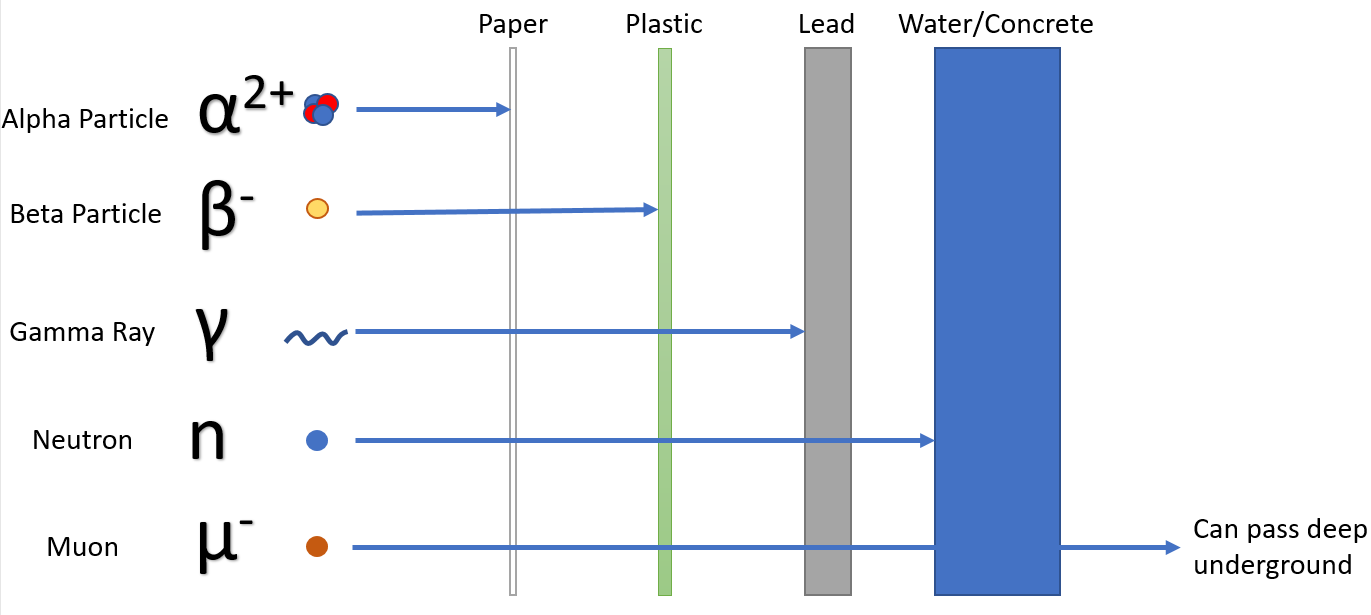
\includegraphics[width=\textwidth]{penetration}
\caption{Various penetration capabilities of several types of radiation}
\label{fig:penetration}
\end{figure}

\subsection{Alpha Particles}
While gamma rays are the dominant type of radiation that germanium detectors are designed to be sensitive to, the other types can still have an effect on measurements and energy spectra.
As shown in Figure \ref{fig:penetration}, alpha particles can be stopped by a thin sheet of paper.
However, they can still interact with the surface of a germanium detector and deposit their energy.
Most alphas would be blocked by the detector housing but some trace amounts of heavy radioactive elements can exist in the metal shielding.
These elements such as uranium 238 or thorium 232 can decay and eject an alpha particle inside the housing that might hit the detector.

As mentioned previously, alpha decay comes from unstable heavy nuclei that spontaneously emit energy in the form of a $^{4}$He nucleus.
The probablity of decay is determined by the barrier penetration mechanism and varies from element to element resulting in half lifes that rande from seconds to thousands of years.
The average kinetic energy of an alpha particle is around 4.6 MeV.
They typically interact through the coulomb force with the electrons in orbit around the absorber atom and can travel aproximately 2.5 cm in air before losing all of its energy.

\subsection{Beta Particles}
Beta particles are more likely than alpha particles to interact with a germanium detector but still unlikely due to them usualy being abosrbed by the detector housing.
Many nuclides decay via beta emission so it is still posible for decays to occur inside the shielding that could hit the detector, or the rare case that a beta would penetrate the housing.
Special detectors can also implement a beryllium window that would facilitate the passage of beta particles to the detector.
Betas lose energy much slower than alpha particles, through both coulomb and radiative processes, so their path through space can be winding and long.
Betas interact with orbital electrons due to them both being negatively charged.


\subsection{Neutrons}
Neutrons have the potential to interact with Ge detectors but due to them having no electric charge, they cannon interact via the coulomb force.
This means they can usually travel many centimeters through material without interacting at all.
For a neutron to deposit energy, it must interact with the nucleus of an atom.

Several classifications exist for neutrons based on the kinetic energy they have and determin which interaction is most likely.
The slowest neutrons are captured by nuclei.
This changes the atomic mass of the atom and can result in a decay which would create a gamma ray.
That gamma ray could then go on to interact with the detector and deposit its energy.
Faster neutrons can scatter off nucleus and deposit some energy.
If a neutron scatters elestically, it gives a nuclear recoil and changes direction.
If it scatters innelastically, it will give a nuclear recoil and can cause and excitation which would result in a gamma ray.
Finally, the fastes neutrons can undergo spallation.
Spallation is when an incoming neutron hits a nucleus and blows it appart and give off massive amounts of energy.

\subsection{Muons}
Muons are negatively charged particles, most of which come from cosmic rays, and are minimum ionizing. 
Muons can travel deep underground and can also create a huge deposition of energy in very short time.
Muons can also spallate.

\subsection{Gamma Rays}
As mentioned earlier, gamma rays are the primary radiation seen by germanium detectors.
Gamma rays have typical energy from 10's of KeV to 2.6 MeV being the highest energy to exist naturally.
Gamma rays can interact with a germanium detector in three ways: through the photoelectric effect, compton scattering, or pair production.
\begin{figure}[htpb]
\centering
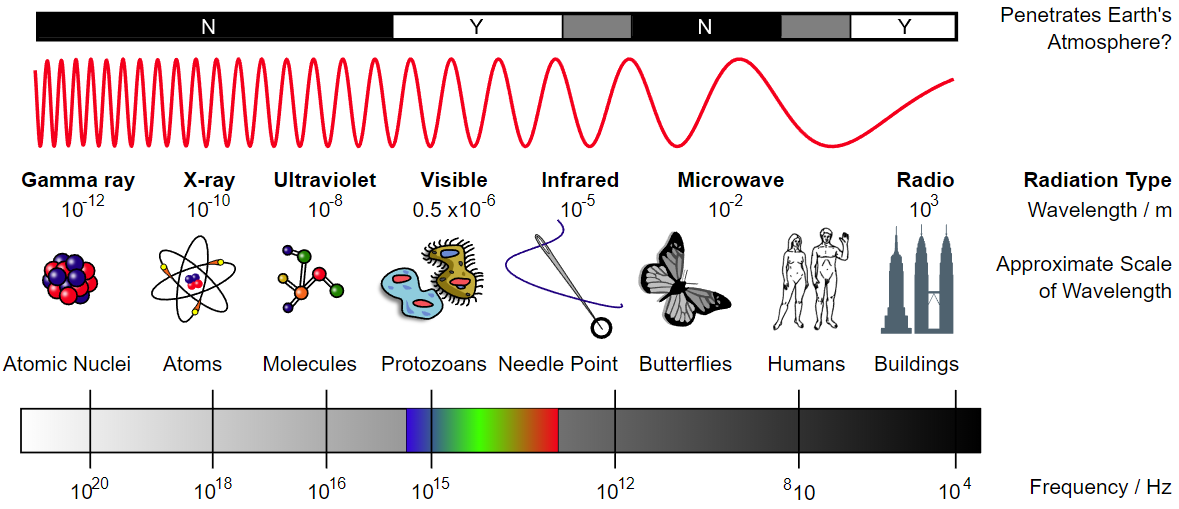
\includegraphics[width=\textwidth]{emspectra}
\caption{Spectrum of electromagnetic waves}
\label{fig:emspectra}
\end{figure}

The photoelectric efect got Einstein a nobel prize and is one of the most important interactions ligt can have with matter.
For the photoelectric effect to occur, an incoming electromagnetic wave must have energy higher than the energy binding the electron to the atom.
If it does, a gamma ray can hit and atom, be abosrbed, and eject an electron with kinetic energy proportional to the incoming gamma ray.
This electron will then wander around losing energy until it is ejected from the surface or stops.
The filling of the hole left by the ejected electron can also cause the emission of characteristic x-ray photons.

The second method, compton scattering, is the most common interaction of germanium detectors and gamma rays.
In compton scattering, the incoming gamma ray is deflected off of an electron to which it transfers some amount of energy.
This recoil electron will then lose energy to the bulk.

The final interation is pair production.
Pair production can occur only if the gamma ray has an energy in excess of twice the rest mass of an electron.
The interaction takes place within the coulomb field of the nucleus and causes the gamma ray to disapear and be replaced by an electron positron pair.
The positron will go on to annihilate which results in the creation of two more gamma rays that could deposit some energy to the detector.
\begin{figure}[htpb]
\centering
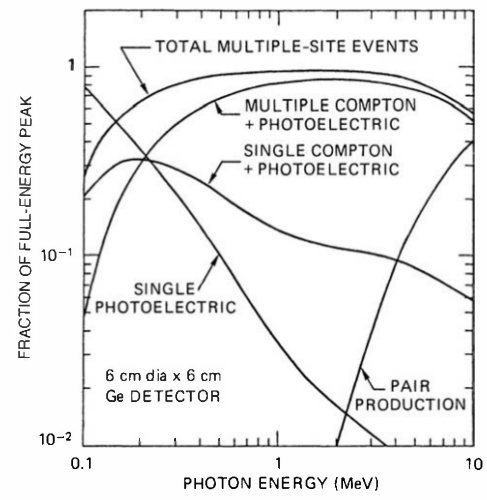
\includegraphics[width=0.4\textwidth]{gammafraction}
  \caption{Fraction of full enrgy peak from different gamma interaction methods in a 6 cm $\times$ 6 cm coaxial HPGe detector expected from a Monte Carlo simulation. \cite{Roth1984SegmentationAP}}
\label{fig:gammafraction}
\end{figure}
Figure \ref{fig:gammafraction} shows the relationship between the various gamma interaction methods and how likely they are to be responsible for the full energy peak obtained during spectroscopy.
It shows that the lowest energy gammas are likely to directly undergo the photoelectric effect and deposit all of their energy.
As the gamma ray energy increases, it is more like to compton scatter at least once before depositing the rest of its energy via the photoelectric effect.
Eventually pair production starts to dominate, however this method only becomes relavent for gamma energies that are typically above those produced by natural radioactivity.

Protons, can behave like a neutron or muon, can interact with EM field or nucleus- might not be needed.

\section{Spectroscopy}
Since a gamma ray is simply a high energy photon, the information we need to decode where it came from is its total energy.
The energy of the gamma rays correspond to specific radioactive elemental decay.
Thus if the entire gamma ray energy can be absorbed and measured by a radiation detector, one can make a reasonable assumption as to the element that it came from.
If a detector is exposed to the environment, gamma rays over a wide distribution of energy with multiple peaks and plateus can be obtained.
The particular interaction of matter and electromagnetic radiation such as a gamma ray is called spectroscopy.

\begin{figure}[htpb]
\centering
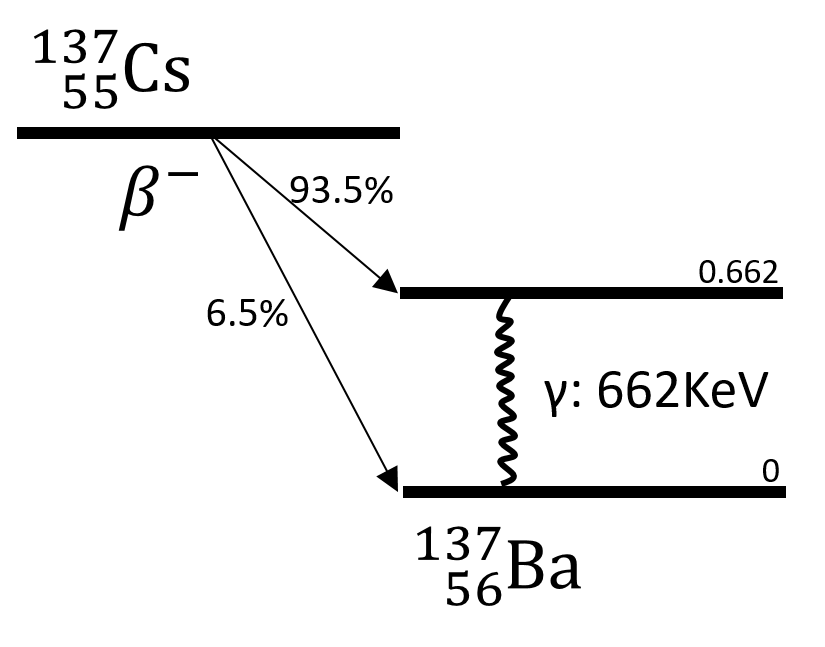
\includegraphics[width=0.5\textwidth]{cs137decay}
\caption{Decay scheme of Cessium 137}
\label{fig:cs137decay}
\end{figure}
An often cited source of gamma radiation is from the man made radioactive isotope Cessium 137.
Cessium 137 is a biproduct of nuclear bomb detonation and has a half life of about 30.166 years \cite{1992NIMPA}.
Cessium 137 decays via beta minus emission as shown in Figure \ref{fig:cs137decay}.
93.5\% of the time this will result in a Barium 137 atom with 662 keV of excess energy that is emitted in the form of a gamma ray.
The other 6.5\% of the time results in the cessium decaying directly to the ground state of barium 137.

Cessium 137 is often used in detector calibration due to the abundance in nature and its single 662 keV gamma ray.
If a source of cessium 137 is placed next to an ionization detector, a spectrum similar to Figure \ref{fig:cs137spectrum} can be obtained.
The spectrum clearly shows a peak inbetween the energy values of 620 and 750 keV.
If the detector could perdectly absorb and measure all of the energy from each gamma ray, it would result in a narrow peak around 662 keV; however, no detector is perfect and statistical flucuations lead to the widening of the peak.
The measure of how precisly a detector can detect energy and read it out is called energy resolution.
\begin{figure}[htpb]
\centering
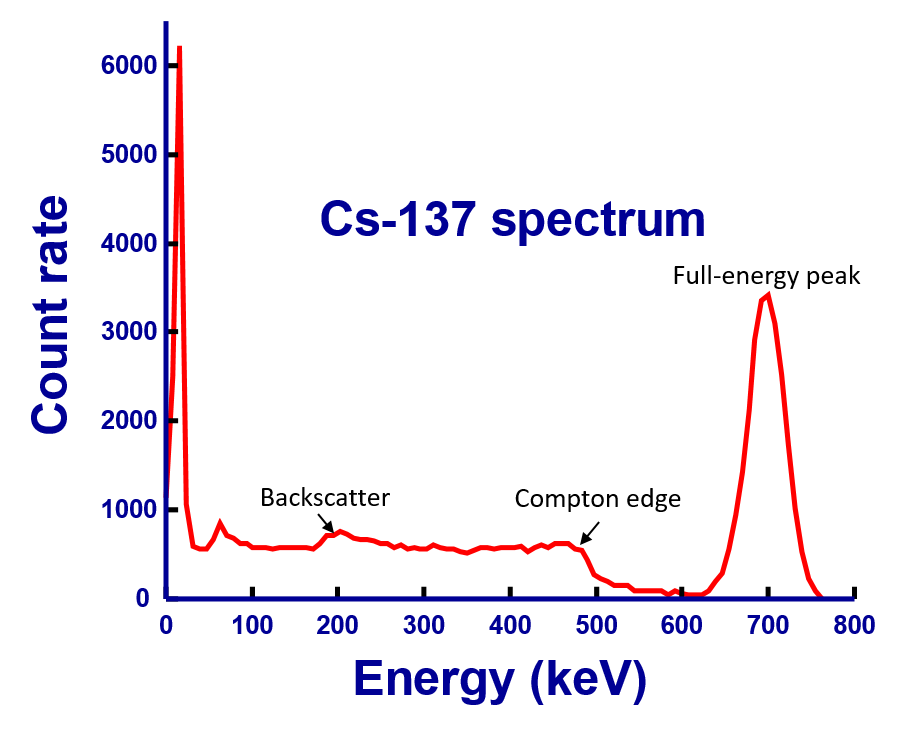
\includegraphics[width=0.7\textwidth]{cs137spectrum}
\caption{Energy spectrum from Cessium 137 using a scintillation based detector \cite{CS137SPEC} translated by Kolbasz}
\label{fig:cs137spectrum}
\end{figure}
The energy resolution of the scintilation detector that was used to obtain the spectrum in Figure \ref{fig:cs137spectrum} is relatively poor due to the wide spread of energy around the known value of 662 keV.

Moving to lower energies on the spectrum, two other features stand out among the background: the compton edge and backscatter peaks.
The compton shoulder is a feature of any detector sensitive to gamma rays and is based on their penetrating nature.
The gamma rays can deposit their energy into a detector via the three methods mentioned in the previous section: photoelectric effect, Compton scattering, or pair production.
Gammas of low energy will undergo the photoelectric effect and deposit all of their energy to the detector; however, according to Figure \ref{fig:gammafraction}, A full energy peak at 662 keV would have less than 10\% of events coming from single photoelectric events.
20\% of the events would be from a single compton scattering event and photoelectric effect, and 70\% would be from multiple compton scattering events ending in photoelectric effect.
Since the dominating interaction is compton scattering, it is clear that some gamma rays could compton scatter inside a detector and then exit without depositing the rest of its energy via photoelectric effect.
Such events would thus only deposit a portion of their energy in the detector resulting in the compton shoulder shown in Figure \ref{fig:cs137spectrum}.

The amount of energy deposited into the detector during a single Compton scattering event is given by the formula:
\begin{align}
  E_c=h\nu \left[ \frac{ \frac{h\nu}{m_0c^2}(1-\cos \theta ) }{1+\frac{h\nu}{m_0c^2}(1-\cos \theta )} \right]
\end{align}
Here $E_c$ is the energy lost by the gamma based on various scattering angles $\theta$ and incoming gamma energy $h\nu$.
The rest mass of the electron $m_0$ is also important as that is what the gamma is scattering off of.
This formula has clear maximum and minum values based on the scattering angle.
A gamma ray that enters the detector and scatters 180 degrees back out would deposit the maximum energy possible in one scattering event.
This value can be calculated for the 662 keV peak from cessium 137.
Plugging in the values of 662 keV for $h\nu$, 1 for $c^2$, 511 keV for $m_0$, and 180 degrees for $\theta$ results in an $E_c$ of 477 keV.
This energy reflects the compton edge from Figure \ref{fig:cs137spectrum}.
The backscatter peak energy can be calculated by subtracting this max value of $E_c$ from the full energy peak value.
In the case of Cessium 137, this would be around 185 keV which also reflects that shown in the cessium spectrum.
Backscatter energies come from gamma rays that have compton scattered off something other than the detector and thus lost a portion of their energy before depositing some or the rest in a detector.

\section{semiconducter diode detector} 
Read all of chapter 11, skip section VI, Channeling
Read chapter 12

Gas vs solid, solid can be hundreds or thousands times more dense than gas so can have smaller detector volume to detect equivalent energy.
Scintilation counters have poor energy resolution due to the small number of information carriers.
Must go from radiation to light to electric signal has a lot of steps where data can be lost and statistical fluctuations on small numbers create a limit to the energy resolution.
In order to reduce the statistical limit is to increase the number of information carriers.
Semiconductor detectors provide increased energy resolution due to more information carriers in terms of electron-hole pairs.
Motion of electron-hole pairs in applied electric field generates the electric signal.
Other advantages to semi conductor detectors: compact size, relatively fast timing charactersistics, and variable effective thickness based on application.
Silicon is used primarily for charged particle spectroscopy while germanium is more widely used in gamma-ray spectroscopy.

band structure
Valence band is made up of the electrons in the outer shell and are bound to specific lattice sites in the crystal.
In germanium they are covalent bonds that make up the interatomic forces within the crystal.
Above the valence band in terms of energy is the conduction band
\begin{figure}[htpb]
\centering
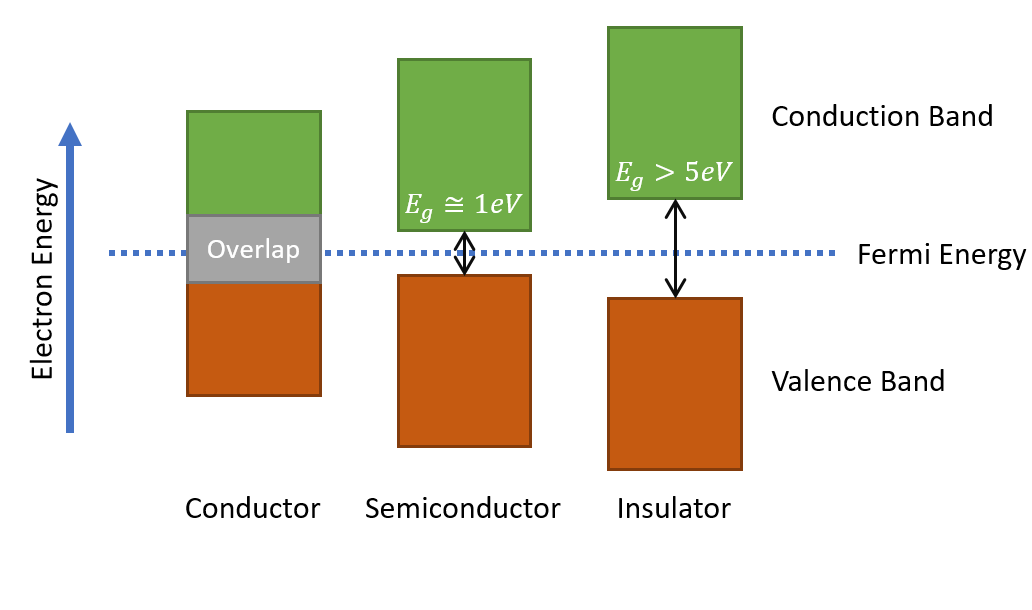
\includegraphics[width=0.9\textwidth]{bandgap}
\caption{Bandgap structures for different material types}
\label{fig:bandgap}
\end{figure}
bands are separated by bandgap
Numer of electrons inside the crystal just fills the valence band
If the bandgap is small enough, electrons can sometimes have enough thermal energy to jump to the conduction band.
This energy comes from the crystal and electrons sharing thermal energy at temperatures above absolute zero.
The electron moving to the conduction band leaves behind an empty spot in the valence band which is called a hole.
If an electric field is applied to the crystal, the electron in the conduction band will drift parallel to the field in the opposite direction.
The hole is also acted upon by the field and will be forced parallel and in the direction of the field.

All materials have some impurities that effect the crystal structure and can take the place of germanium atoms.
Some of them have electrons in the outer shells that exceed the amount required by the crystal lattice (4) and are thus weakly bonded.
It will not leave a hole behind when it is moved to the conduction band
Impurities of this type are called donor impurities and if a crystal is doped with excess donor atoms on the order of $10^{10}$ cm$^{-3}$
If a material is doped with atoms that have less electrons than required by the lattice, such as those from group III of the periodic table, there will be an extra hole avalaible to be filled.
The is called an acceptor site
\begin{figure}[htpb]
\centering
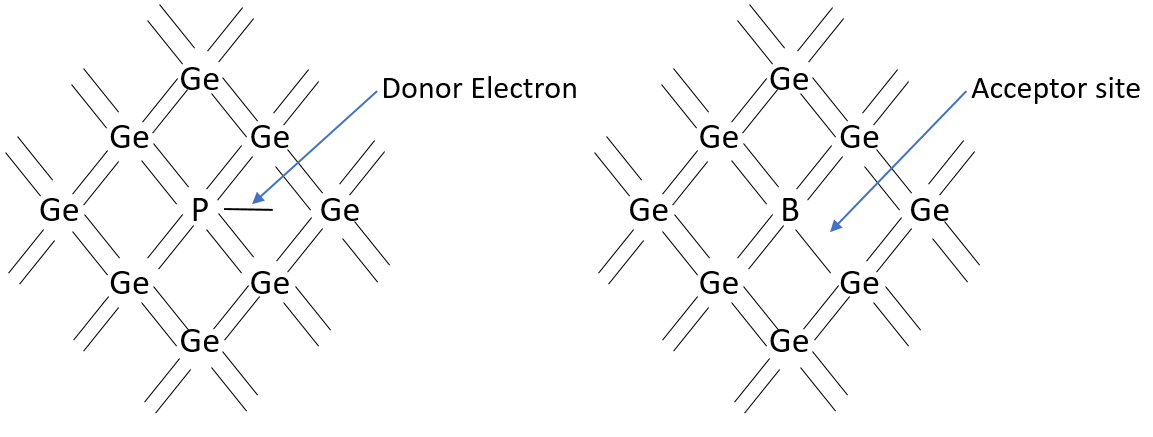
\includegraphics[width=\textwidth]{type}
\caption{Left: example of donor impurity configuration. Right: Example of acceptor impurity configuration}
\label{fig:type}
\end{figure}
An electron can fill an acceptor site where it will be left with a looser bond than the bulk of the crystal.
Whatever carrier is dominant determines the type of material.
Materials where electrons are the majority carrier, such as those doped with phosphorous, are called n-type semiconductors.
When the holes are the dominant information carrier, such as germanium doped with boron, the material is
 called p-type.

The energy required to create one electron hole pair is called the ionization energy $\epsilon$.
When a charged particle travels through a detector it creates electron-hole pairs along its path
There are always equal numbers of electrons and holes created within a few picoseconds
Both carriers need to be fully collected in order to get an accurate energy measurement

For the semiconductor to be a detector, there needs to be a way of collecting the charge generated by an event.
A typical event that generates that loses 1 MeV of energy will generate around $3\times 10^{5}$ electron hole pairs.
If all were drifted with an electric field and collected, it would only generate a current pulse of around $10^{-6}$A.
There needs to be a sufficiently low current through the detector, such that when electron hole pairs are created, the added current pulse can be measured.
Thus it is necessary to have some sort of carrier blocking electrodes.
This will limit the amount of injected charge and current flowing through the bulk of the detector and bring the leakage current to sufficiently low levels.
Leakage current of the system needs to be on the order of $10^{-9}$A in order to be sufficiently low to not interfere with the radiation induced pulse.

